%!TEX root = ../Thesis.tex
\section{UserStories \& Use Cases}

\subsection*{Nicolas Groß}

Ich als Gamer möchte sehen, welche die beliebtesten Spiele auf Steam sind. Gleichzeitig möchte ich ohne großen Aufwand eines der beliebten Spiele kaufen. Dabei möchte ich aber Geld sparen und kaufe deshalb einen Spielelizenzschlüssel (Key). Ich möchte die Angebote nicht einzeln vergleichen, sondern alle Angebote nebeneinander aufgelistet haben, um den günstigsten Anbieter zu finden. Dann möchte ich per Click an diesen Weitergeleitet werden.


\begin{figure}[hbt]
    %\centering
    \begin{minipage}[t]{1\textwidth} % Breite, z.B. 1\textwidth		
        \caption{Use Case Authentifizieren} % Überschrift
        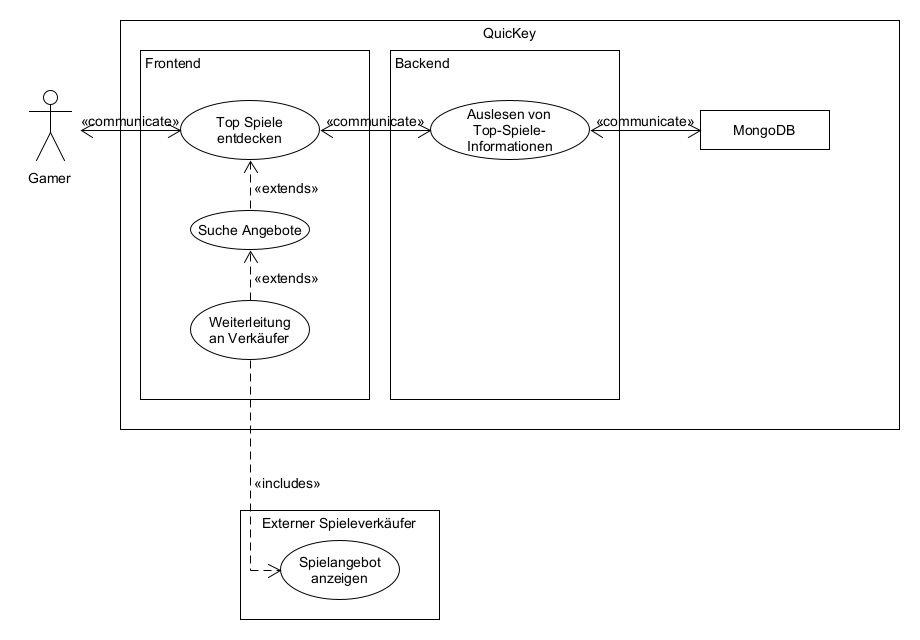
\includegraphics[width=1\textwidth]{img/use_case_gamer.png}\\ % Pfad
        \source{Eigene Darstellung} % Quelle
    \end{minipage}
\end{figure}
\newpage
\subsection*{Niklas Hardes}

Ein Kunde möchte eine persönliche Liste von Spielen anlegen können, mit den für ihn beliebtesten Spielen. Dadurch kann er mit wenig Aufwand diese schnell auf Ihren aktuellen Preis überprüfen. 

\begin{figure}[hbt]
    %\centering
    \begin{minipage}[t]{.7\textwidth} % Breite, z.B. 1\textwidth		
        \caption{Use Case Authentifizieren} % Überschrift
        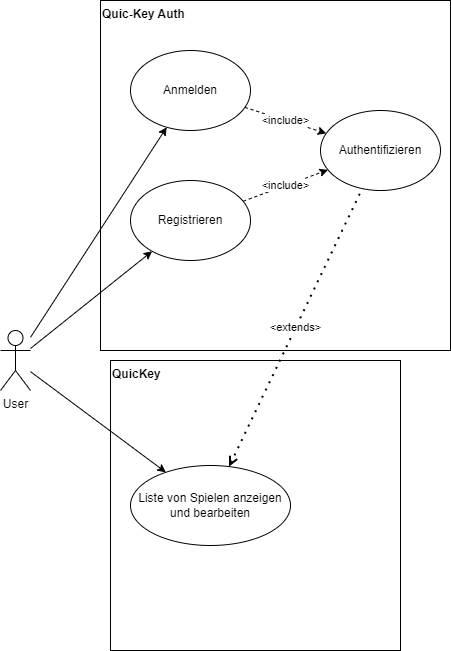
\includegraphics[width=1\textwidth]{img/use_case_auth.png}\\ % Pfad
        \source{Eigene Darstellung} % Quelle
    \end{minipage}
\end{figure}
\newpage
\subsection*{Robert Hesselmann}

Ein erfolgreicher Streamer auf der Livestreaming Plattform Twitch sucht nach neuen Spielen, die er in seinen Livestreams spielen kann. Um seinen Gewinn zu maximieren sucht er nach einem Spiel zu einem günstigen Preis.

\begin{figure}[hbt]
    %\centering
    \begin{minipage}[t]{.7\textwidth} % Breite, z.B. 1\textwidth		
        \caption{Use Case Streamer} % Überschrift
        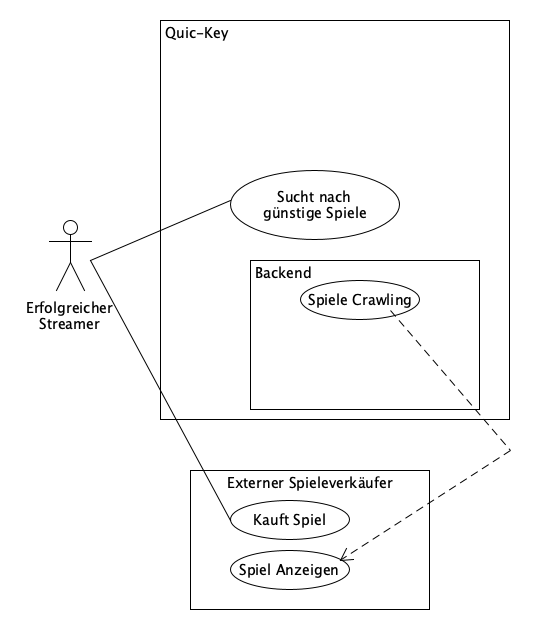
\includegraphics[width=1\textwidth]{img/use_case_streamer.png}\\ % Pfad
        \source{Eigene Darstellung} % Quelle
    \end{minipage}
\end{figure}
    
